\chapter{Special Tasks Cookbook}

Siehe DevelManual

\section{Creating Colormaps}

\subsection{ParaView}
\url{http://www.itk.org/Wiki/Manually_Creating_a_Colormap}

\begin{figure}[htp]
  \begin{center}
    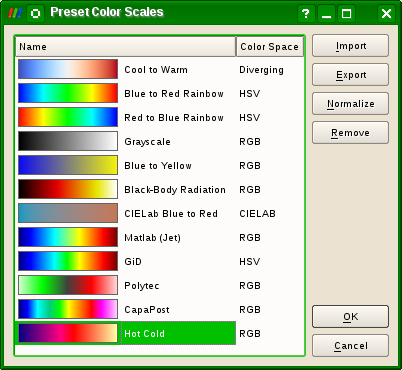
\includegraphics[height=4cm]{pics/pv_colormaps} 
  \end{center}
  \caption{Predefined colormaps from ParaView and CFS++.}
  \label{fig:cfs_pv_colormaps}
\end{figure}


\subsection{Gnuplot}
\url{http://gnuplot.sourceforge.net/demo/pm3dcolors.html}

\subsection{Matlab}
\url{http://www.mathworks.de/help/techdoc/ref/colormap.html}
\url{http://www.mathworks.de/help/techdoc/ref/colormapeditor.html}


\section{Lighting Options}

\subsection{ParaView}
No Lighting

\begin{figure}[htp]
  \begin{center}
    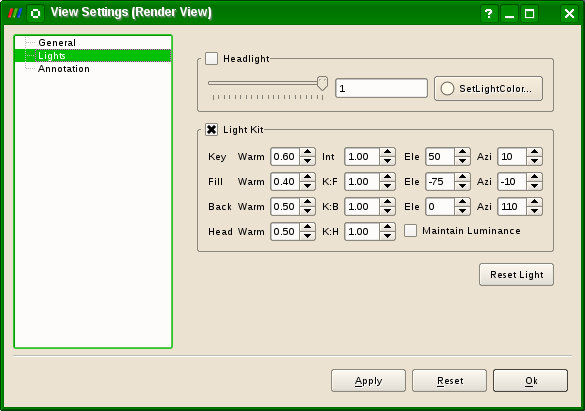
\includegraphics[height=4cm]{pics/pv_nolight} 
  \end{center}
  \caption{Predefined colormaps from ParaView and CFS++.}
  \label{fig:cfs_pv_colormaps}
\end{figure}

\begin{figure}[htp]
  \begin{center}
    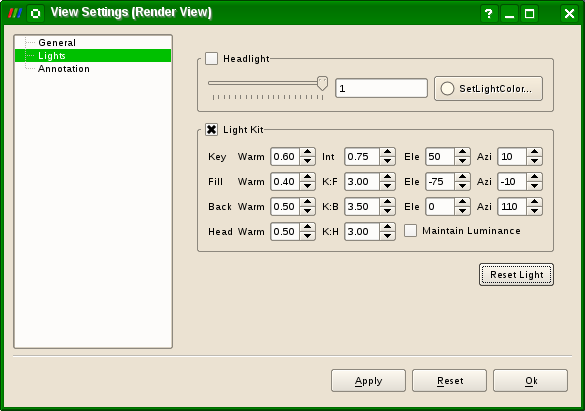
\includegraphics[height=4cm]{pics/pv_light_default} 
  \end{center}
  \caption{Predefined colormaps from ParaView and CFS++.}
  \label{fig:cfs_pv_colormaps}
\end{figure}

\begin{figure}[htp]
  \begin{center}
    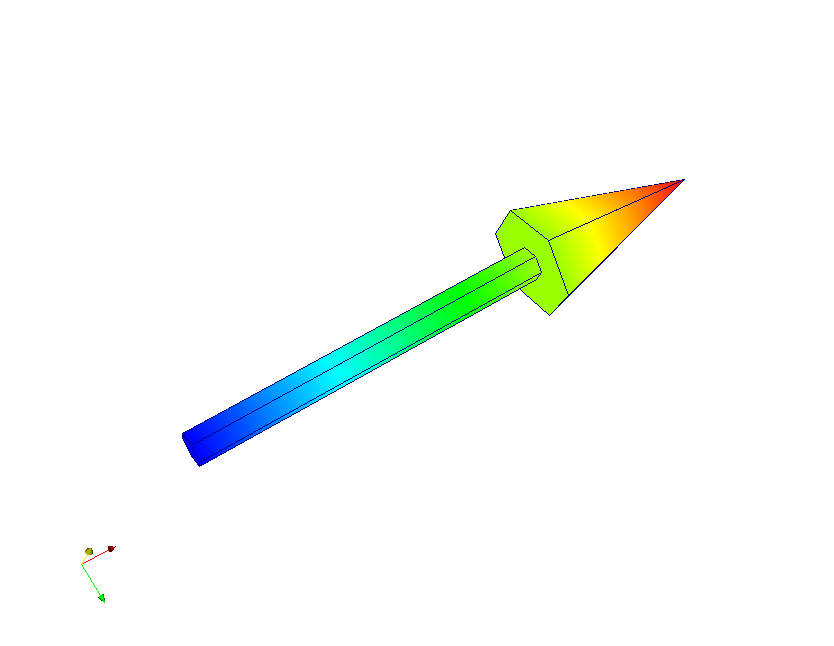
\includegraphics[height=4cm]{pics/pv_nolight_arrow} 
  \end{center}
  \caption{Predefined colormaps from ParaView and CFS++.}
  \label{fig:cfs_pv_colormaps}
\end{figure}

\begin{figure}[htp]
  \begin{center}
    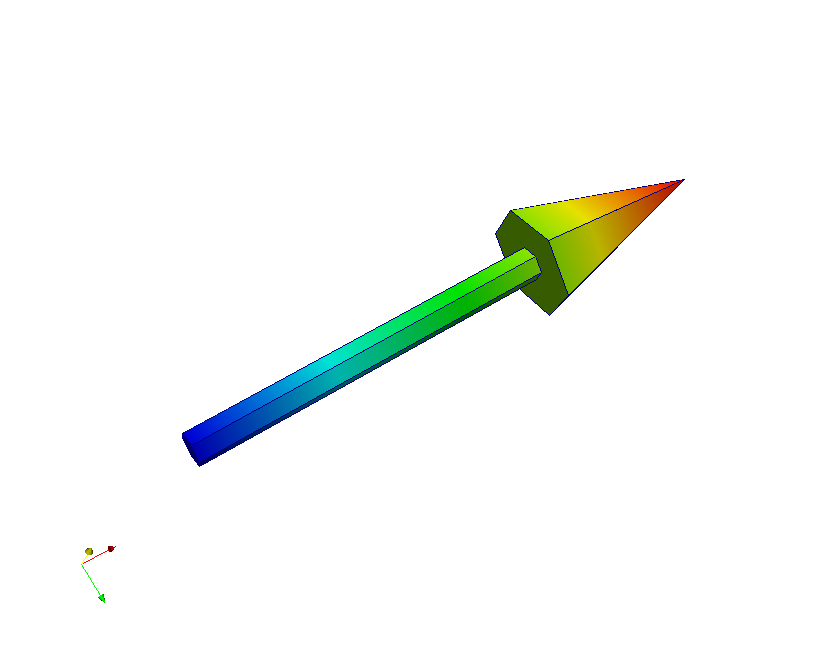
\includegraphics[height=4cm]{pics/pv_light_default_arrow} 
  \end{center}
  \caption{Predefined colormaps from ParaView and CFS++.}
  \label{fig:cfs_pv_colormaps}
\end{figure}
